
\subsection*{New potential and repulsive Coulomb interaction}


Introducing a new potential $V_{\rho} = \omega^2\rho^2 + \frac{1}{\rho}$ where $\omega$ is an oscillator frequency and $\frac{1}{\rho}$ is a repulsive Coulomb potential. First considering the value of $\rho_{max}$ in the case without a repulsive Coulumb interaction. Where finding a value of $\rho_{max}$ so that the eigenvalues are stable is the first step. \fxnote{rewrite sentence}  
%----------------------------------
\begin{wraptable}{r}{5.0cm}
\caption{hei hei\fxnote{add caption}} 
\label{tab:rhomax}
\phantom{.}
\begin{tabular}{|c|c|c|}
\hline
$\rho_{max}$ & N & 3rd eigenvalue \\
\hline 
1 & 10 & 83.5237 \\
2 & 20 & 21.8365 \\
3 & 30 & 9.79411 \\
4 & 40 & 5.5277 \\
\vdots & \vdots & \vdots \\
9 & 90 & 1.0983 \\
10 & 100 & 0.890899 \\
10.1 & 101 & 0.873488 \\
11 & 110 & 0.737631 \\
\hline

\end{tabular}

\end{wraptable}
%------------------------------------
For this to be stable the change should be small, so $\rho_{max} = 10$ and the change is about 0.2 between the surrounding steps. Also the change between 10 and 10.1 is about 0.02 so small changes in $\rho_{max} $ doesn't give big changes. Also the relation between $\rho_{max}$ and n is kept constant so that \fxnote{ref h} is constant. Running for different values of $\rho_{max}$ with the ratio gives \tabref{tab:rhomax}, which shows that when $\rho_{max} $ is 10 the results are stable for the 3rd eigenvalue. The reason for choosing the 3rd eigenvalue is that it is more sensitive for change of $\rho_{max}$ and it's the last printed eigenvalue in the program. 


The Eigenvectors are used for determining the wave function, and in this case they are used squared so they show the probability density of the distance $\rho$ between the two electrons. Which gives the most probable distance between the particles,the distance $\rho = (\frac{1}{\alpha})r$ where $\alpha = (\frac{\hbar^2}{mk})^{1/4}$. The reason for this is better described in \secref{sec:NatureOfTheProblem}. Plotting the distance as a function of $\rho$ for different values of the frequency $\omega_r$, \figref{fig:ProbFuncOmegaWithout} shows that for a higher frequency $\omega_r$ the distance between the particles are bigger and the spread in area which the particle can be in is also more stretched out. 

\begin{figure}[H]
	\centering
	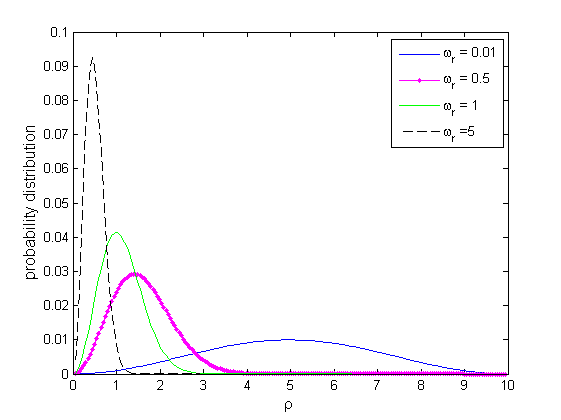
\includegraphics[width=0.75\textwidth]{Figures/2particles_without.png}
	\caption{The probability density as a function of distance $\rho$ without repulsive Coulomb interaction. Where $\rho_{min} = 0$, $\rho_{max} = 10$ and $n = 200$  }
	\label{fig:ProbFuncOmegaWithout}
\end{figure}

When adding a repulsive Coulomb potential $\frac{1}{\rho}$ to the potential $V(\rho )$ in \figref{fig:ProbFuncOmega} the probability density is pushed to a longer distance, although it might be a bit difficult to see in \figref{fig:ProbFuncOmega} and \figref{fig:ProbFuncOmegaWithout}.

\begin{figure}[H]
	\centering
	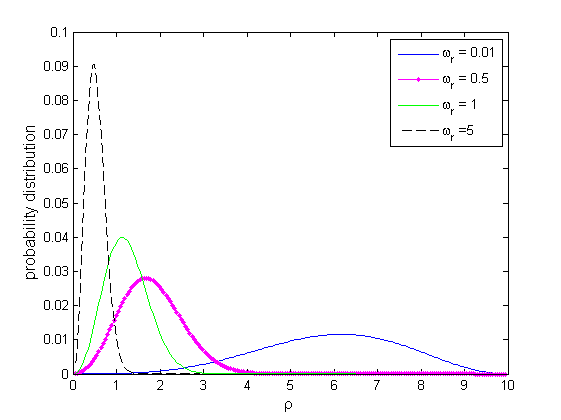
\includegraphics[width=0.75\textwidth]{Figures/ProbFuncOmega.png}
	\caption{The probability density as a function of distance $\rho$ with a repulsive Coulomb interaction. Where $\rho_{min} = 0$, $\rho_{max} = 10$ and $n = 200$}
	\label{fig:ProbFuncOmega}
\end{figure}





